%version of 07-03-18

\chapter{SUMMATION}
\label{ch:Summation}


\section{Introduction}
\label{sec:intro}

The operation of {\it summation}---adding up aggregates of
numbers---is of fundamental importance in the world of digital
computing.  While we humans are able to deal handily with abstractions
such as ``smoothness'' and ``continuity'', we must employ
sophisticated {\em discretizations} of these concepts in order to
enlist the aid of digital computers in dealing with such abstractions.
Summations provide a very useful discretization of ``continuous'' or
``smooth'' phenomena that are typically dealt with by humans with the
aid of the (differential and integral) calculus that was invented by
Newton and Leibniz for such dealings.

This chapter is dedicated to exploring how to employ summations as a
computational tool.  We deal throughout with {\it series}, {\it i.e.},
(possibly infinite) sequences of numbers
\[ a_1, a_2, \ldots \]
whose sum
\begin{equation}
\label{eq:abstract-sum}
a_1 + a_2 + \cdots
\end{equation}
is of interest.
\begin{quote}
{\em Of course, when we deal with {\em infinite} series, wherein there
  are infinitely many numbers $a_i$, we must address the question of
  whether the sum (\ref{eq:abstract-sum}) exists as a finite number.
  For some infinite series the sum {\em does} exist as a finite
  number, as with the well-known sum
\[ 1 \ + \ \frac{1}{2} \ + \ \frac{1}{4} \ + \ \frac{1}{8} \ +
\ \frac{1}{16} \ + \ \cdots \ + \ \frac{1}{2^k}  \ +
\ \frac{1}{2^{k+1}} \ + \ \cdots \ = \ 2 
\]
%{\Denis Here we can refer to the Achille and Tortoise story as this corresponds to the distance Achille's did to reach the tortoise if the initial situation is 1 meter...}
(Such an infinite series is said to {\em converge}.)
\index{infinite series!convergent}

But sometimes an infinite series {\em does not} have a finite
  sum.  This is true, for instance, with the well-known {\it harmonic}
  series \index{harmonic series}
\[ 1 \ + \ \frac{1}{2} \ + \ \frac{1}{3} \ + \ \frac{1}{4} \ +
\ \frac{1}{5} \ + \ \cdots \ + \ \frac{1}{k}  \ + \ \frac{1}{k+1} \ +
\ \cdots
\]
As more and more terms are added, the accumulated sum eventually
passes every number.  (Such an infinite series is said to {\em diverge}.)
{\Denis There is a link between harmonic series and the frequencies of the notes in music (each note corresponds to the fundamental divided by 2, 3, 4, ...
May be it would be nice here to develop?}
{\Arny I do not know enough to say anything intelligent about this.}
\index{infinite series!divergent}
}
\end{quote}

\begin{quote}
We note parenthetically that the preceding sum illustrates some of the
complexity of dealing with the infinite.  Sometimes finite objects
(such as the integer $2$ in this example) have infinite ``names'' (the
infinite series in this example).  The complexity of the concept of
convergence has been recognized in various forms for more than $25$
centuries.  Several charming and familiar examples appear in the
paradoxes attributed to Zeno of Elea.  In his {\it Paradox of Achilles
  and the Tortoise}, for instance, Zeno appears to prove that all
motion is illusory.  In this story, the slow-footed Tortoise (T) tries
to convince the speedy Achilles (A) of the futility of trying to win
any race in which A gives T even the smallest head start.  As long as
T is ahead of A, says T, every time A traverses half the distance
between the competitors, T will respond by moving a bit further ahead.
Thereby, T will always be a positive distance ahead of A, so that A
can catch T.  A similar ``argument'' demonstrates that an arrow shot
at you by an adversary can never reach you, as long as you continually
move away from the archer.  {\em DO NOT TRY THIS AT HOME!!}

The subtleties of the notion of {\em infinitesimals} that explains the
fallacy of assertions such as the Tortoise's was not well understood
until a few hundred years ago.
\end{quote}


Toward the end of guiding the reader through the forest of
abstractions and operations and techniques associate with summations,
we categorize the targets of our discussions in three ways.
\begin{enumerate}
\item
We study a number of {\it fundamental sums} that have intrinsic
interest.
%{\Denis Notice here that none of the following examples are arithmetic or geometric...}
Examples of this category of topic include {\it arithmetic sums}, {\it
  geometric sums}, and {\it mathematically ``smooth'' sums}, including
sums of positive and negative powers, such as the following:
\[
\begin{array}{lcl}
1 \ + \ 2 \ + \ 3 \ + \ 4 \ + \ 5 \ + & \cdots & + \ k  \ + \ (k+1) \ +
\ \cdots \ + \ n \\
1 \ + \ 2 \ + \ 4 \ + \ 8 \ + \ 16 \ + & \cdots & + \ 2^k  \ +
\ 2^{k+1} \ + \ \cdots \ + \ 2^n \\
1 \ + \ 4 \ + \ 9 \ + \ 16 \ + \ 25 \ + & \cdots & + \ k^2  \ + \ (k+1)^2 \ +
\ \cdots \ + \ n^2 \\
1 \ + \ \frac{1}{2} \ + \ \frac{1}{4} \ + \ \frac{1}{16} \ +
\ \frac{1}{32} \ + & \cdots & + \ \frac{1}{2^k}  \ + \ \frac{1}{2^{k+1}} \ +
\ \cdots \\
1 \ + \ \frac{1}{2} \ + \ \frac{1}{3} \ + \ \frac{1}{4} \ +
\ \frac{1}{5} \ + & \cdots & + \ \frac{1}{k}  \ + \ \frac{1}{k+1} \ +
\ \cdots \\
1 \ + \ \frac{1}{4} \ + \ \frac{1}{9} \ + \ \frac{1}{16} \ +
\ \frac{1}{25} \ + & \cdots & + \ \frac{1}{k^2}  \ + \ \frac{1}{(k+1)^2} \ +
\ \cdots
\end{array}
\]

\item
We study a variety of {\it fundamental techniques} for performing
summations.

We include specialized techniques that work for specific classes of
summations, as well as more general techniques that work in a broad
range of situations.

Examples of such techniques include, e.g.: estimating summations by
integrating functions related to the summation; grouping/replication
of terms within a summation; verifying ``guessed'' sums via induction.

\item
We study a variety of {\it fundamental representations} of the
elements be summed.  We find that being able to study the same
phenomenon in a variety of seemingly unrelated ways often give one
unexpected mathematical control over the phenomenon.

Examples of such representations include, e.g., representing numbers
by: numerals in a positional number system; Riemann sums; slices of
pie; tokens arranged in stylized ways; and basic geometrical
structures.
\end{enumerate}

{\em In summation, we treat each topic in multiple ways, as long as
  each new way teaches the reader a new lesson.}

\bigskip

%%%%%%%%%%%%%%%%%%%%%%%%%%%%%%%%%%%%%%%%%%%%%%%%





\ignore{\Denis Again, as I said before, I am not really convinced by this example.
Keeping the same sum, I prefer the story of Sissa, telling an old legende:
where wheat or rice is placed upon each square of the chess board in the following way:
put one grain on the first square, and then, double this number on each of the subsequent squares,
$2$ in the second case, $4$ in the third and so on.}

\ignore{\Denis add cross reference for computing the sum of powers of 2 in DOINGMATHS}

To illustrate the power of summation methodology, consider the
following modernized version of the {\it legend of Sissa ibn Dahir}.
\index{Sissa ibn Dahir, legend of}
You have invented a marvelous game, let's call it {\it chess}, that is
played on an $8 \times 8$ array of unit-size squares---call it a {\it
  chessboard}.  A benefactor offers you a one-time gift of {\em one
  million million (i.e., $10^{12} = 1,000,000,000,000$) euros} in
return for all rights to the game.  As a counter-offer, you ask your
benefactor instead for all of the money amassed in the following way.
You ask your benefactor to proceed row by row along the chessboard,
placing money in the squares, according to the following regimen.
Your benefactor should place $1$ euro in the first square, $2$ euros
in the second square, $4 \ (= 2 \times 2)$ euros in the third, $8 \ (=
4 \times 2)$ euros in the third , and so on, doubling the number of
euros at each step of the procedure---so the last square would contain
$2^{64}$ euros.

\noindent
{\em Have you made a good bargain?}

\medskip

By the end of this chapter, you will be able to determine in minutes
that under your procedure (the one that uses the chessboard), you
would receive $2^{65} -1$ euros---which is {\em much} more than
$10^{20}$ euros!
%{\Denis I think the previous value is -1 and not -2}

\noindent
{\em A good bargain, indeed!}

%%%%%%%%%%%%%%%%%%%%%%%%%%%%%%%%%%%%%%%%%%%%%%%%%%%%


\section{Summing Structured Series}
\label{sec:structured-series}

\subsection{Arithmetic Sums and Series}
\label{sec:arithmetic-series}

\subsubsection{General development}

We define arithmetic sequences and learn how to calculate their sums.

\begin{equation}
\label{eq:arith-seq}
\begin{array}{l}
\mbox{An $n$-term arithmetic sequence:} \\
\hspace*{.25in}a, \ a+b, \ a+2b, \ a+3b, \ \ldots, a+(n-1)b \\
\\
\mbox{The corresponding arithmetic series:} \\
\hspace*{.25in}a + (a+b) + (a+2b) + (a+3b) + \cdots + (a+(n-1)b) \\
\hspace*{.5in} = \
an + b \cdot (1 + 2 + \cdots + n-1)
\end{array}
\end{equation}
We can, thus, sum the arithmetic series in (\ref{eq:arith-seq}) by
determining the sum of the first $m$ positive integers; $m = n-1$ in
(\ref{eq:arith-seq}).  We use this result as an opportunity to
introduce important notation.

\subsubsection{Special cases}

%\addcontentsline{toc}{paragraph}{A. Case study: Summing the first $n$ integers}

\paragraph{\small\sf A. Summing the first $n$ integers: the case $a=b=1$}.
%The sum is denoted by $\Delta_n$.

\begin{prop}
\label{thm:sum-first-integers-Gauss}
\index{sum of first $n$ integers}
For all $n \in \N$,
\begin{eqnarray}
\nonumber
S_1(n) \ \eqdef \ \sum_{i=1}^n \ i \
  & \eqdef &
 1 + 2 + \cdots + (n-1) + n \\
\label{eq:sum-1-to-n}
  & = & \frac{1}{2} n (n+1) 
% \\
%\nonumber 
%  & = & {{n+1}  \choose 2}.
\end{eqnarray}
\end{prop}

%{\Denis I removed the last equality with n+1 choose 2 since this
%combinatorial proof is presented later...}

\begin{proof}
{\bf A textual proof.}
\index{sum of first $n$ integers!a textual reckoning}
%
We begin with a {\em constructive} proof\footnote{The proof is {\em
    constructive} in that it actually derives an answer.  This is in
  contrast to, say, the inductive validation of the sum in
  Section~\ref{sec:positive-integer-power}.C, which just verifies a
  ``guessed'' answer.}~of summation (\ref{eq:sum-1-to-n}) that employs
an approach known to the eminent German mathematician Karl Friedrich
Gauss \index{Gauss, Karl Friedrich} as a pre-teenager.  \index{Gauss,
  Karl Friedrich!summation ``trick''} This approach proceeds in two
steps.
\begin{equation}
\label{eq:arith-series}
\begin{array}{llccccccccc}
\mbox{Write $S_1(n)$ ``forwards'':} &
\hspace*{.2in}\sum_{i=1}^n \ i \ = & 1 & + & 2   & + & \cdots & + & (n-1) & + & n \\
 & & & & & & & & & &  \\
\mbox{Write $S_1(n)$ ``in reverse'':} &
\hspace*{.2in}\sum_{i=n}^1 \ i \ = & n & + & (n-1) & + & \cdots & + & 2   & + & 1
\end{array}
\end{equation}
Now add the two representations of $S_1(n)$ in (\ref{eq:arith-series})
{\em columnwise}.  Because each of the $n$ column-sums equals $n+1$,
we find that $2 S_1(n) = n(n+1)$, which we easily rewrite in the form
(\ref{eq:sum-1-to-n}) (after multiplying both sides of the equation by
$2$).
\end{proof}

\medskip

\noindent {\bf Remark.}
%
{\em Now is an opportune moment to step back from the specific result
  proved in Proposition~\ref{thm:sum-first-integers-Gauss} and
  concentrate on the textual proof.  What Gauss noticed about the sum
  of the first $n$ integers is that when the sum is doubly written as
  in (\ref{eq:arith-series}), the column-sums are all the same.  This
  phenomenon of {\em finding invariants} is a ``pattern'' of the form
  referred to in Section~\ref{sec:manifesto} as we discussed how
  mathematicians ``do mathematics''.  We see in the proof how the
  pattern can be exploited to determine sum of any arithmetic series.
  {\em What seemed to be a ``trick'' turns out to be an insightful
    instance of pattern-matching.}  We show now that the pattern can
  be exploited to other, related, ends.}

\medskip

Not everyone thinks the same way---even within the context of
mathematics.  It is, therefore, very important for the reader to
recognize that even the simplest mathematical facts can be proved and
analyzed in a broad variety of ways.  We illustrate this assertion by
developing two more proofs of
Proposition~\ref{thm:sum-first-integers-Gauss}.

\begin{proof}
{\bf A ``pictorial'', graphic proof.}
\index{sum of first $n$ integers!a ``pictorial'', graphic reckoning}
%
The idea now is to look at the problem of summing the first $n$
integers as a problem of estimating the area of a simple (in the
\textit{good sense} of the word) surface.  In this worldview, integers
are represented by concatenating basic {\it unit-side} (i.e., $1
\times 1$ \index{unit-side square} {\it squares}), as in
Fig.~\ref{fig:sumIntegersGeo1}.

Our summation result can be obtained in three steps, in the manner
illustrated by the three figures
Figs.~\ref{fig:sumIntegersGeo1},~\ref{fig:sumIntegersGeo2},
and~\ref{fig:sumIntegersGeo3}.
\begin{figure}[h]
\begin{center}
       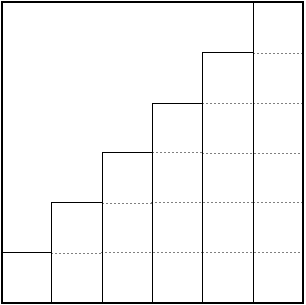
\includegraphics[scale=0.4]{FiguresMaths/SumIntegersGeometricBasis}
\caption{Representing the first $n$ integers using basic unit squares; $n=6$ in this example.}
       \label{fig:sumIntegersGeo1}
\end{center}
\end{figure}
\begin{figure}[h]
\begin{center}
       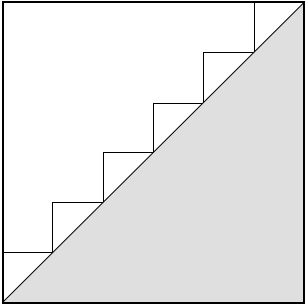
\includegraphics[scale=0.4]{FiguresMaths/SumIntegersGeometricIntermediate}
\caption{The area of the lower-right triangle (light grey) is one-half that of
  the entire $n \times n$ square.}
       \label{fig:sumIntegersGeo2}
\end{center}
\end{figure}
\begin{figure}[h]
\begin{center}
       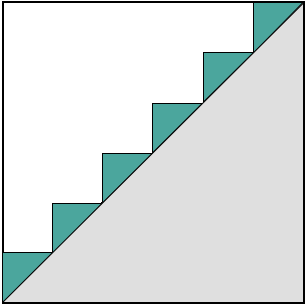
\includegraphics[scale=0.4]{FiguresMaths/SumIntegersGeometricFinal}
\caption{The area of the (dark) triangles sitting on the upper
  diagonal of the $n \times n$ square is $\frac{1}{2} n$.}
       \label{fig:sumIntegersGeo3}
\end{center}
\end{figure}
\begin{enumerate}
\item
To begin, in Fig.~\ref{fig:sumIntegersGeo1} we depict the problem of
summing the first $n$ integers as the problem of determining the area
of a surface constructed from unit-side squares.

\item
Next, we illustrate in Fig.~\ref{fig:sumIntegersGeo2} that the area of
the lower-right triangle of the $n \times n$ square---depicted in
light grey in the figure---is one-half that of the entire $n \times n$
square.

\item
Finally, we indicate in Fig.~\ref{fig:sumIntegersGeo3} that the area
of the small (dark grey in the figure) triangles that cover the upper
diagonal of the $n \times n$ square is $\frac{1}{2} n$.  This
reckoning is because there are $n$ triangles, and each has an area that
is one-half that of a unit-side square.
\end{enumerate}
We thereby reckon the area of the surface depicting the summation as

\begin{tabular}{l}
{\it One-half the area of the $n \times n$ square,
i.e., $\frac{1}{2} n^2$} \\
\hspace*{.15in} plus   \\
{\it $n$ times the area of one-half a unit-side square,
i.e., $\frac{1}{2} n$}
\end{tabular}

\noindent
We have, thus determined the value of $S_1(n)$.
\end{proof}

\medskip

We present one final proof of
Proposition~\ref{thm:sum-first-integers-Gauss}.

\begin{proof}
{\bf A combinatorial proof.}
\index{sum of first $n$ integers!a A combinatorial reckoning}
%
The following argument is {\it combinatorial} in that it achieves its
goal by {\em counting} instances of the first $n$ integers, laid out
in a line.

Place (tokens that represent) the integers $0$ to $n$ along a line.
For each integer $i$, count how many integers $j > i$ lie to its
right.  We see that in general, there is a {\it block} of $n-i$
integers that lie to the right of integer $i$.  In detail: the block
of integers lying to the right of $i=0$ contains $n$ values of $j$;
the block to the right of $i=1$ contains $n-1$ values of $j$, and so
on, as suggested in Fig.~\ref{fig:rightward-instances}.

\begin{figure}[htb]
\[
\begin{array}{lcccccc}
\mbox{All integers $\leq 4$:} &
 & 0 & 1 & 2 & 3 & 4 \\
\mbox{integers to the right of $0$:} &
 &   & 1 & 2 & 3 & 4 \\
\mbox{integers to the right of $1$:} &
 &   &   & 2 & 3 & 4 \\
\mbox{integers to the right of $2$:} &
 &   &   &   & 3 & 4 \\
\mbox{integers to the right of $3$:} &
 &   &   &   &   & 4
\end{array}
\]
\caption{A two-dimensional depiction of the right-lying
  integer-instances.}
\label{fig:rightward-instances}
\end{figure}

On the one hand, we see that the total number of right-lying integers
$j$ equals $n+(n-1)+ ... + 1 \ = \ S_1(n)$.

On the other hand, every instance of a right-lying integer can be
identified uniquely by the pair of nonnegative integers, $i$ (the
instance's block) and $j>i$ (the instance's position-within-block).
The total number of right-lying integer-instances corresponds to the
number of ways to select two integers from among $n+1$.\footnote{We
  study such counting techniques in depth in
  Section~\ref{sec:counting}.}  This number is the binomial
coefficient $\Delta_{n}$ whose definition we specialize from
(\ref{eq:binom-coeff}) Section~\ref{sec:binary-operators}.C:
\index{binomial coefficient}
\[ 
\Delta_n \ = \ {{n+1} \choose 2} \ \eqdef \ \frac{1}{2} n(n+1).
\]

We have thus arrived at two, perforce equal, expressions for $S_1(n)$.
\end{proof}

\medskip

Now that we know---via several arguments---the value of $S_1(n)$, we
can finally evaluate our original series in (\ref{eq:arith-seq}).
\index{arithmetic series:explicit sum}

\begin{prop}
\label{thm:sum-of-arithmetic-series}
The arithmetic series in (\ref{eq:arith-seq}) has the sum
\[
a + (a+b) + (a+2b) + (a+3b) + \cdots + (a+(n-1)b) \ = \
%an + b \cdot {n \choose 2}. 
an + b \cdot \Delta_n. 
\]
\end{prop}


\paragraph{\small\sf B. Perfect squares are sums of odd integers}

We now build on Proposition~\ref{thm:sum-first-integers-Gauss} to
craft {\em two} constructive proofs that each perfect square, say,
$m^2$, is the sum of the first $m$ odd integers, $1, 3, 5, \ldots,
2m-1$.  (This is again an arithmetic series with $a=1$ and $b=2$.)
One of these proofs builds on the phenomenon of {\em finding
  invariants}.  These proofs complement the ``guess-and-verify''
inductive proof of the same result in
Section~\ref{sec:positive-integer-power}.C.

\begin{prop}
\label{thm:squares-odd-integers-Gauss}
\index{$n^2$ as sum of first $n$ odd integers}
For all $n \in \N^+$,
\begin{equation}
\label{eq:sum-of-odds}
\sum_{k=1}^n \ (2k-1)
 \ = \ 1 + 3 + 5 + \cdots + (2n-1) \ = \ n^2.
\end{equation}
That, is, the $n$th perfect square is the sum of the first $n$ odd
integers.
\end{prop}

Before presenting our two proofs of this result, we note that the
notation in (\ref{eq:sum-of-odds}) is perfectly general: every positive
odd integer $m$ can be written in the form $2n-1$ for some positive
integer $n$.
{\Denis According to the expression of Proposition~\ref{thm:sum-of-arithmetic-series},
the sum is equal to $1.n + 2 \Delta_{n-1} = n + n^2 -n = n^2$.
Let us detail several alternative proofs.}

\smallskip

\begin{proof}
{\bf A textual proof.}
%
Let us adapt Gauss's ``trick'' to this problem.  Let us denote the
target sum $\sum_{k=1}^n \ (2k-1)$ by $S(n)$. 
\begin{equation}
\label{eq:add-odds}
\begin{array}{llccccccccc}
\mbox{$S_n$ ``forwards'':} &
S(n) \ = 
& 1 & + & 3 & + & \cdots & + & (2n-3) & + & (2n-1) \\
 & & & & & & & & & &  \\
\mbox{$S_n$ ``in reverse'':} &
S(n) \ =
& (2n-1) & + & (2n-3) & + & \cdots & + & 3 & + & 1
\end{array}
\end{equation}
Now add the two representations of $S(n)$ in (\ref{eq:add-odds}) {\em
  columnwise}.  Because each of the $n$ column-sums equals $2n$, we
find that
\begin{equation}
\label{eq:sum-of-odds-sum}
2 S(n) \ = \ 2 \sum_{k=1}^n \ (2k-1) \ = \ 2n^2.
\end{equation}
We thus derive the desired summation (\ref{eq:sum-of-odds}) when we
divide both sides of equation (\ref{eq:sum-of-odds-sum}) by $2$.
\end{proof}

\medskip

\begin{proof}
{\bf A proof using algebra.}
%
Our second proof derives this result, via a simple calculation, as a
corollary of Proposition~\ref{thm:sum-first-integers-Gauss}.

By direct calculation, we have
\begin{eqnarray*}
\sum_{k=1}^n \ \left( 2k-1 \right)
   & = & 2 \sum_{k=1}^n \ k \ \ - \ n \\
   & = & 2 \frac{n (n+1)}{2} \ \ - \ n \ \ \ \ \mbox{ by
  Proposition~\ref{thm:sum-first-integers-Gauss}} \\
   & = & (n^2 + n) - n \\
   & = & n^2.
\end{eqnarray*}
\end{proof}

\medskip

Our next proof is purely pictorial, with a bit of reasoning mixed in.
The only ``sophisticated'' required background knowledge is that
\[ (n+1)^2 \ = \ n^2 \ + \ 2n \ + \ 1. \]
This simplest instance of the {\em restricted Binomial
  Theorem}---which appears later in this chapter as
Theorem~\ref{thm:restricted-binomial-thm}---can be verified using the
highly perspicuous Fig.~\ref{fig:proofa2plusb2}.
%{\Denis We can remark here that this result is straightforward as
%follows. see below if you think it should be included.}
\begin{figure}[h]
\begin{center}
       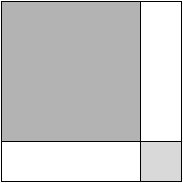
\includegraphics[scale=0.4]{FiguresMaths/proofa2plusb2}
\caption{A geometrical proof of the identity $(n+1)^2 = n^2 + 2n + 1$.}
       \label{fig:proofa2plusb2}
\end{center}
\end{figure}
The figure tells its tale by means of four rectangles that make up an
$(n+1) \times (n+1)$ square, whose area is, of course, $(n+1)^2$.
This large square is made up of four rectangles.  Reading across the
top of the figure, we encounter a darkly shaded $n \times n$ square
(area $= n^2$) and an unshaded $n \times 1$ rectangle (area $= n$).
Reading across the bottom of the figure, we encounter an unshaded $1
\times n$ rectangle (area $= n$) and a lightly shaded $1 \times 1$
square (area = $1$).  The overall message is that

\noindent
$(n+1)^2$ (the area of the large, composite, square)

\begin{tabular}{ll}
is the sum of & \\
  & $n^2$ (the area of the darkly shaded square) \\
plus & \\
  & $2n$ (the combined areas of the unshaded rectangles \\
plus & \\
  & $1$ (the area of the lightly shaded square)
\end{tabular}

\medskip

\noindent
Back to Proposition~\ref{thm:squares-odd-integers-Gauss}.

\begin{proof}
{\bf A proof ``by pictures''.}
%
Our pictorial proof begins by representing an integer $n$ as a
horizontal sequence of $n$ ``bullets'', i.e., dark circles.  The
problem of summing the first $n$ odd integers then begins with a
picture such as appears in Fig.~\ref{fig:sumOdds1}, for the
illustrative case $n=5$.
\begin{figure}[h]
\begin{center}
       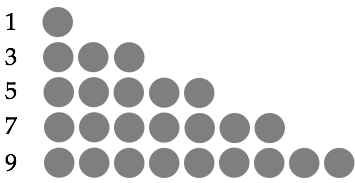
\includegraphics[scale=0.4]{FiguresMaths/SumOddsBasis}
\caption{Representing the first $n$ odd integers using bullets.  In
  this illustration, $n=5$.}
       \label{fig:sumOdds1}
\end{center}
\end{figure}

Starting with such a picture, we take each row of $2c+1$ bullets and
fold it at its midpoint so that it becomes a reversed letter ``$L$''.  The
row of $2c+1$ bullets becomes an ``$L$'' whose horizontal portion (at the
bottom of the reversed ``$L$'') is a row of $c+1$ bullets and whose
vertical portion (at the right of the reversed ``$L$'') is a column of
$c+1$ bullets.  See Fig.~\ref{fig:sumOdds2} wherein the depicted
values of $c$ are $c = 0, 1, 2, 3, 4$.
\begin{figure}[h]
\begin{center}
       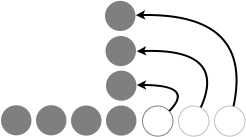
\includegraphics[scale=0.4]{FiguresMaths/SumOddsIntermediate}
              \caption{Folding a single row into a reversed letter ``$L$''.}
       \label{fig:sumOdds2}
\end{center}
\end{figure}

Once we have folded every row of bullets into a reversed ``$L$'', we nest
the ``$L$''s in the manner depicted in Fig~\ref{fig:sumOdds3}.
\begin{figure}[h]
\begin{center}
       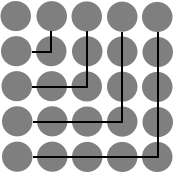
\includegraphics[scale=0.4]{FiguresMaths/SumOddsFinal}
\caption{The final picture organized as an $n \times n$ square
  array of bullets.}
       \label{fig:sumOdds3}
\end{center}
\end{figure}
Clearly, this nesting produces an $n \times n$ square array of
(perforce, $n^2$) bullets.
\end{proof}

\medskip

\begin{proof}
{\bf A proof by rearranging terms.}
%
We describe in Section~\ref{sec:Fubini} how the Italian mathematician
Guido Fubini
\index{Fubini, Guido}
%
was able to make notable mathematical progress by rearranging
representations \cite{Fubini}.  Within the context of the current
chapter, such rearrangements work on the terms of a summation of
interest.  Indeed, using this strategy, we obtain a surprising,
delightful proof of Proposition~\ref{thm:squares-odd-integers-Gauss}.
Let us take the odd integers in order, in groups of sizes $1$, then
$2$, then $3$, and so on.  We begin with the first $n$ odd integers in
order:
\[ 1, \ 3, \ 5, \ 7, \ 9, \ 11, \ 13, \ 15, \ 17, \ 19, \ \ldots \]
Now we start peeling off prefixes of successive numbers of odd
integers and arranging them in an array, as depicted in
Table~\ref{tab:SumOddsTriangle}.
\begin{table}[h]
\label{tab:SumOddsTriangle}
\caption{The sums of successive odd numbers and the sum of
  successive cubes}
\[
\begin{array}{llrrrrclcc}
\mbox{group of size 1:} & &
1,  &    &     &     &  \rightarrow & 1           & = & 1^3 \\
\mbox{group of size 2:} & &
3,  &  5, &     &    &  \rightarrow & 2 \times 4  & = & 2^3 \\
\mbox{group of size 3:} & &
7,  &  9, & 11, &    &  \rightarrow & 3 \times 9  & = & 3^3 \\
\mbox{group of size 4:} & &
13, & 15, & 17, & 19 &  \rightarrow & 4 \times 16 & = & 4^3 \\
\end{array}
\]
\end{table}
What we note is that---at least with the illustrated portion of the
procedure---the $k$th group, of size $k$, adds up to $k^3$.

Before we proceed further, let us verify---by induction---that this
pattern persists indefinitely.
\begin{description}
\item[{\small\sf Base for the induction.}]
The trivial one-term entry in row $1$ of Table~\ref{tab:SumOddsTriangle}
provides the base for our induction.

\item[{\small\sf Inductive hypothesis}.]
We know from Proposition~\ref{thm:sum-first-integers-Gauss} that the
$k$th group consists of $k$ consecutive odd numbers beginning with
\[ 2 \Delta_{k-1} +1 \ \ \ \ \
\mbox{which is the} \ \ \ \ \
\left( \Delta_{k-1} +1 \right)\mbox{th odd number}
\]
Hence, this group begins with $2 \Delta_{k-1} +1$ and ends with
$2\Delta_k -1$.
%{\Denis the right expression is: beginning with $2\Delta_{k-1} +1$ and ending at $2\Delta_k-1$}

%{\Denis I prefer to refer to $\Delta_k$ instead of ${k+1 \choose 2} $... }

This proof can be represented graphically as follows.  We begin with
the unit square (the leftmost item in Fig.~\ref{fig:sumCubes1}) as the
basis of our induction.
\begin{figure}[h]
\begin{center}
       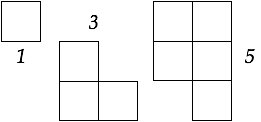
\includegraphics[scale=0.4]{FiguresMaths/SumCubes1}
\caption{The basis for the inductive pictorial proof}
       \label{fig:sumCubes1}
\end{center}
\end{figure}
We next represent the number $2^3$ (the {\em cube} of $2$) by two $2
\times 2$ squares: the figures following the unit square in
Fig.~\ref{fig:sumCubes1}.
\begin{figure}[h]
\begin{center}
       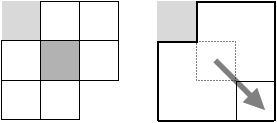
\includegraphics[scale=0.4]{FiguresMaths/SumCubes2}
\caption{Showing graphically that $2^3 +1$ is a perfect square}
       \label{fig:sumCubes2}
\end{center}
\end{figure}
Fig.~\ref{fig:sumCubes2} illustrates graphically that $1+ 2^3$
is a perfect square.
\begin{figure}[h]
\begin{center}
       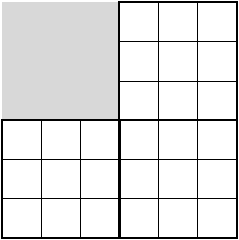
\includegraphics[scale=0.4]{FiguresMaths/SumCubes3}
\caption{The next step in the construction also produces a perfect square}
       \label{fig:sumCubes3}
\end{center}
\end{figure}
Fig.~\ref{fig:sumCubes3} illustrates that iterating the process also
produces a perfect square.  Comparing Figs.~\ref{fig:sumCubes2}
and~\ref{fig:sumCubes3} indicates a parity constraint on the process:
at even-numbered steps,the subsquares that get ``merged'' are
overlapping; at odd-numbered steps, they are not.


\item[{\bf Inductive extension}.]
%
Since successive odd numbers differ by $2$, we know that the $k$th
group consists of the following odd integers ($k>1$):
\[
2 \Delta_{k-1} +1, \ 2 \Delta_{k-1}  +3, \ 2 \Delta_{k-1}  +5 ,
\ldots, \
2 \Delta_{k-1} +2k-1
\]
\ignore{One verifies easily (say, by induction) that $2 \Delta_{k-1} +2k-1 = 2
\Delta_{k} +1$.
Hence, this group has the sum}
\[
2k {k \choose 2} \ - \ 2 {k \choose 2} +k \ = \
(2k -1) \Delta_k + k \ = \ k^3.
\]
\end{description}

%{\Denis here is my solution... Please, check}

Because each row contains one more integer than its predecessor, row
$k$ contains the sum of the odd integers from $\Delta_{k-1}+1$ to
$\Delta_k$.  By direct calculation, we can therefore compute the row's
sum as
\[
\left( \frac{k(k+1)}{2} \right)^2 \ - \ \left( \frac{k(k-1)}{2} \right)^2
 \ \ =  \ \ \frac{k^2}{4} \left( (k+1)^2 - (k-1)^2 \right)
% & = & \frac{k^2}{4} (4k) \\
 \ \ = \ \ k^3
\]
\end{proof}

We close this treatment with another, really basic proof.  As stated
earlier, our goal is really to encourage readers to utilize every
possible mathematical concept as they hone their mathematical and
computational skills.

\begin{proof}
{\bf A final proof, from elementary school.}
%
Consider the following reasoning which emerges from the way
multipication tables are developed in elementary school.  We
illustrate the idea using the case $n=5$.
\[
\begin{array}{rrrrr}
1  &  2 &  3 &  4 &  5 \\
2  &  4 &  6 &  8 & 10 \\
3  &  6 &  9 & 12 & 15 \\
4  &  8 & 12 & 16 & 20 \\
5  & 10 & 15 & 20 & 25 \\
\end{array}
\]
Write the integers $1, 2, \ldots, n$ in a row.  Below this row, write
the doubles of these integers.  The next row holds the triples of the
integers; then come the quadruples of the integers, then the
quintuples, and so on.  Note that the resulting table is symmetric:
its rows are identical to its columns.

Using Fubini's rearrangement stratagem, we count all the integers in
the table in two different ways.
\begin{enumerate}
\item
We sum the entries of our table by peeling away successively larger
reversed instances of the letter ``$L$'' (as in our earlier
``pictorial'' proof of
Proposition~\ref{thm:squares-odd-integers-Gauss}).  We find that the
integers in each ``$L$'' sum to a perfect cube:
\[
\begin{array}{ccccccccc|cl}
1  &    &    &    &    &   &     &    &   & 1   & = 1^3 \\
2  &  4 &  2 &    &    &   &     &    &   & 8   & = 2^3 \\
3  &  6 &  9 &  6 &  3 &   &     &    &   & 27  & = 3^3 \\
4  &  8 & 12 & 16 & 12 &  8 &  4 &    &   & 64  & = 4^3 \\
5  & 10 & 15 & 20 & 25 & 20 & 15 & 10 & 5 & 125 & = 5^3
\end{array}
\]

\item
We sum the successive rows of our previous $n$ by $n$ table.  The first rowof the table
sums to $\Delta_n$; the second sums sums to $2 \Delta_n$; the third
sums to $3 \Delta_n$, \ldots; the last row sums to $n \Delta_n$.
Thus, the total sum is $(1 + 2 + \cdots + n) \Delta_n \ =
\ \left(\Delta_n \right)^2$.
\end{enumerate}
We conclude that
\[
\sum_{i=1}^n i^3 \ = \  \left(\Delta_n \right)^2
\]
\end{proof}

\ignore{\Arny More calculation!  BOO!  Please complete this.  I seem to be off by 1}
%We give another proof that tells us something more on numbers of their interactions.
%We consider numbers instead of bullets, and we use a similar principle as Fubini, that is to determine a
%suitable organization of the numbers and count them in a simple way.
%For the concern of computing the sum of the first odd numbers, we organize them as shown in Table~\ref{tab:SumOddsTriangle}.
%One number in the first row, two in the second, $k$ on the $k$th row.
%There are $\Delta_p$ (complete) rows. 
%The result is obtained by summing up the elements of each row.
%The sum in a row is equal to the perfect cube of this row.
%This result can be easily proven. 
%{\Denis Should I develop here? or we can let it as an exercice?}
%

\medskip

In Section~\ref{sec:sum-of-i2c>0}, we shall see the underpinnings of 
techniques that incrementally compute the sums of the first $n$
consecutive integers, squares of integers, cubes of integers, and so
on, i.e., that compute the sums for $k$th powers from the sums for
smaller powers.

\paragraph{\small\sf C. Another application of arithmetic sums}

Let us consider $a=1$ and $b=4$. 
The sum is $S(n)=n+4 \Delta_{n-1}$.
From the arrangement given in Fig.~\ref{fig:Delta(n)4}, it is easy to see that it is equal to $\Delta_{2n-1}$ (4 triangles of size $n$ plus a row of $n$ bullets in dark grey
form a bigger triangle of size $2n-1$).
\begin{figure}[h]
\begin{center}
       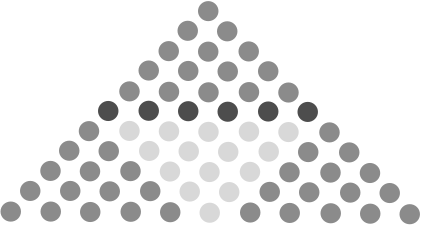
\includegraphics[scale=0.5]{FiguresMaths/Delta(n)4}
 \caption{Arranging the four triangles plus a row to obtain a new (bigger) triangle.}
       \label{fig:Delta(n)4}
\end{center}
\end{figure}

%%%%%%%%%%%%%%%%%%%%%%%%%%%%%%%%%%%%%%%%%%%%%%%%%%%%

\subsection{Geometric Sums and Series}
\label{sec:geometric-sums}


\subsubsection{General development}
\label{sec:general-geometric}

We define geometric sequences and learn how to calculate their sums
via the following generic example.
\index{geometric sequence}
\index{geometric series}
\begin{equation}
\label{eq:geom-seq}
\begin{array}{l}
\mbox{An $n$-term geometric sequence:} \\
\hspace*{.25in}a, \ ab, \ ab^2, \ \ldots, ab^{n-1} \\
 \\
\mbox{The corresponding geometric series:} \\
\hspace*{.25in}a + ab + ab^2 + \cdots + ab^{n-1} \ = \
 a (1+ b + b^2 + \cdots + b^{n-1})
\end{array}
\end{equation}
It is clear just from this definition that we can sum the series in
(\ref{eq:geom-seq}) by summing just the sub-series
\begin{equation}
\label{eq:geom-series}
S_{b}(n) \ \eqdef \
1+ b + b^2 + \cdots + b^{n-1}.
\end{equation}

Along the way to developing a solution technique for the series
$S_{b}(n)$, we will uncover an even simpler solution
technique that that establishes the following.

\begin{prop}
\label{thm:sum-infinite-geometric-series}
When $b < 1$,  the {\em infinite} series
\[ \sum_{i=0}^\infty \ b^i \ = \ 1 + b + b^2 + \cdots \]
sums to $\displaystyle \frac{1}{1-b}$.
\end{prop}

\bigskip

For general values of $b$ and general limits of summation, we have the
following slightly more cumbersome analogue of
Proposition~\ref{thm:sum-infinite-geometric-series}; that simpler
proposition follows as a corollary of the following.

\begin{prop}
\label{thm:sum-finite-geometric-series}
Let $S_{b}(n)$ be an arbitrary geometric sum, as defined in
(\ref{eq:geom-series}).

\noindent {\bf (a)}
When $b > 1$, $S_{b}(n)$ evaluates to the following sum.
\begin{equation}
\label{eq:geom-sum:b>1}
S^{b>1}_{b}(n) \ = \ \frac{b^{n}- 1}{b - 1}.
\end{equation}

\noindent {\bf (b)}
When $b < 1$, $S_{b}(n)$ evaluates to the following sum.
\begin{equation}
\label{eq:geom-sum:b<1}
S^{b<1}_{b}(n) \ = \ \frac{1 - b^n}{1-b}.
\end{equation}

\noindent {\bf (c)}
Note that when $b < 1$, the {\em infinite} version of $S_b(n)$,
namely, $\sum_{i=0}^\infty b_i$ is a {\em convergent} series with the
following sum
\[ S_b^{(\infty)} \ \eqdef \sum_{i=0}^\infty b_i \ = \ \frac{1}{1-b} \]
\end{prop}

Of course, the uninteresting degenerate case $b=1$ sums to $n$.

\begin{proof}
{\bf A proof by textual replication.}
%
Toward the end of developing our first method for summing $S_{b}(n)$,
we note that we can rewrite the sum in two ways that are {\em
  (textually) recurrent}.

\bigskip

\noindent
{\em This phenomenon of {\em finding recurrent subexpressions} is a
  ``pattern'' of the form referred to in Section~\ref{sec:manifesto}
  as we discussed how mathematicians ``do mathematics''.  We now
  exemplify how this pattern can be exploited to find explicit sums
  for geometric series.}

\bigskip

Both of the recurrent expressions for $S_{b}(n)$ have the following form.
\begin{equation}
\label{eq:geom-series-recurrent}
S_b(n) \ = \ \alpha \cdot S_b(n) \ + \ \beta(n)
\end{equation}
where $\alpha$ is a constant and $\beta(n)$ is a function of $n$; both
$\alpha$ and $\beta(n)$ may depend on the parameter $b$.
\begin{equation}
\label{eq:geom-series-replicate}
\begin{array}{cclcl}
S_{b}(n) 
  & = &
1+ b + b^2 + \cdots + b^{n-1} & & \\
  &   &   &  & \\
  & = &
1 + b \cdot S_{b}(n) - b^n
   & = & b \cdot S_{b}(n) \ + \ (1 - b^n) \\
  &   &   &  & \\
  & = &
{\displaystyle
b^{n-1} + \frac{1}{b} \cdot S_{b}(n) - \frac{1}{b}
}
  & = &
{\displaystyle \frac{1}{b} \cdot S_{b}(n) \ + \ \frac{b^n -1}{b} 
}
\end{array}
\end{equation}
The significance of a recurrent expression of the form
(\ref{eq:geom-series-recurrent}) is that it exposes an explicit value
for $S_b(n)$:
\begin{equation}
\label{eq:geom-series-generic}
S_b(n) \ = \ \frac{\beta(n)}{1 - \alpha}
\end{equation}

We can now combine the generic value (\ref{eq:geom-series-generic}) of
$S_b(n)$ with the specialized recurrent expressions for $S_b(n)$ in
(\ref{eq:geom-series-replicate}) to derive two explicit solutions for
$S_b(n)$.
\begin{enumerate}
\item
The first solution is most useful and perspicuous when $b>1$.  In this
case, we find that
\[ \left( 1 - \frac{1}{b} \right)  S^{b>1}_{b}(n) \ = \ b^{n-1} -
\frac{1}{b}, \]
which can easily be rearranged to the equivalent and more
perspicuous form (\ref{eq:geom-sum:b>1}).

\item
The second solution is most useful and perspicuous when $b < 1$.  In this
case, we find that
\[ (1-b) S^{b<1}_{b}(n) \ = \ 1 \ - \ b^n \]
which can easily be rearranged to the equivalent and more
perspicuous form (\ref{eq:geom-sum:b<1}).
\end{enumerate}
\end{proof}

Note that both $S^{b>1}_{b}(n)$ and $S^{b<1}_{b}(n)$ have simple {\em
  approximate} values which are useful in ``back-of-the-envelope''
calculations: For very large values of $n$, we have
\begin{equation}
\label{eq:geom-sum:approx}
S^{b>1}_{b}(n) \ \approx \ \frac{b^n}{b-1} \ \ \
\mbox{while} \ \ \
S^{b<1}_{b}(n) \ \approx \ \frac{1}{1-b} .
\end{equation}
The expression for $S^{b<1}_{b}(n)$ in (\ref{eq:geom-sum:approx}) is
actually a rewording of
Proposition~\ref{thm:sum-infinite-geometric-series}.

\medskip

\begin{proof}
{\bf A pictorial proof of Proposition~\ref{thm:sum-infinite-geometric-series}.}
%
Fig.~\ref{fig:sumGeoBasis} depicts a pictorial process whose analysis
provides a rigorous argument that $\displaystyle \sum_{i=0}^\infty
\ 2^{-i}$ evaluates to $2$ (as promised by
Proposition~\ref{thm:sum-infinite-geometric-series}).
\begin{figure}[h]
\begin{center}
       \includegraphics[scale=0.4]{FiguresMaths/SumGeometric1sur2Bis}
 \caption{Arranging successive rectangles to sum $\displaystyle
   \sum_{i=0}^\infty \ 2^{-i}$.}
       \label{fig:sumGeoBasis}
\end{center}
\end{figure}
We measure fractional quantities by the portion of a unit-side
rectangle that they fill.  Thus (follow in the figure): The initial
term of $\displaystyle \sum_{i=0}^\infty \ 2^{-i}$, namely $1$, is
represented by the unit square that is labeled ``$1$'' in the figure.
The next term of the series, namely $1/2$, is represented by the
rectangle labeled ``$1/2$'' in the figure.  We proceed with
successively smaller rectangles representing successively smaller
inverse powers of $2$.  As the process proceeds, we observe
increasingly more of the righthand unit-side square being filled.  In
fact, one can argue that {\em every} point in the righthand square
eventually gets covered by some small rectangle (as $n$ tends to
$\infty$), thereby establishing that the infinite series
$\displaystyle \sum_{i=0}^\infty \ 2^{-i}$ sums to $2$.

\ignore{*******
The result is immediate while considering a basic unit square and its
successive decompositions while divided by $2$.
Thus, the whole surface corresponds to the sum of $(\frac{1}{2})^k$. 
It is equal to $2$ (surface of the two big squares) and it is completely filled. 
***********}

This procedure is hard---but not impossible---to adapt to values of $b
<1$ other than $\frac{1}{2}$.
\begin{figure}[h]
\begin{center}
       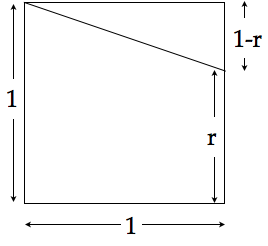
\includegraphics[scale=0.4]{FiguresMaths/SumGeometricGeneral1}
\caption{Initial state: the unit square and $r$.}
       \label{fig:sumGeoGeneral1}
\end{center}
\end{figure}
\begin{figure}[h]
\begin{center}
       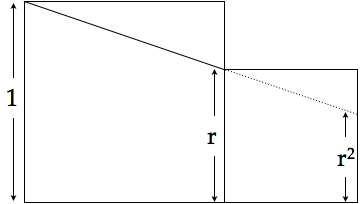
\includegraphics[scale=0.4]{FiguresMaths/SumGeometricGeneral2}
\caption{Geometric series obtained by an appropriate cascading of
  shrinking squares.}
       \label{fig:sumGeoGeneral2}
\end{center}
\end{figure}
Fig.~\ref{fig:sumGeoGeneral3} suggests how to achieve such an
adaptation for any value of $b$ with $0 \leq b <1$, by an
appropriately chosen cascade of shrinking squares.
\begin{figure}[h]
\begin{center}
       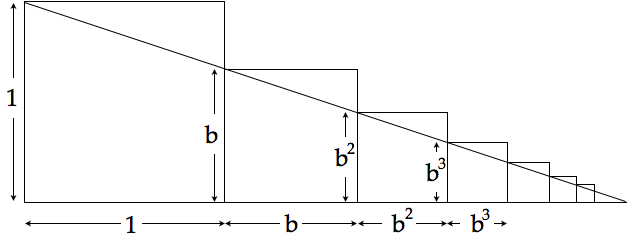
\includegraphics[scale=0.4]{FiguresMaths/SumGeometricGeneral3}
\caption{The complete process for computing a geometric series via a
  cascade of shrinking squares.}
       \label{fig:sumGeoGeneral3}
\end{center}
\end{figure}
The lengths of the bases of the abutting rectangles is the value of
the infinite series $\displaystyle \sum_{i=0}^\infty \ b^{-i}$.
\end{proof}



\subsubsection{An extension and an application}
\label{sec:extended-geom-series}

\paragraph{\small\sf A. On summing ``extended'' geometric series}

We now build on our sums (\ref{eq:geom-sum:b>1},
\ref{eq:geom-sum:b<1}) for geometric series to evaluate what we shall
call ``extended'' geometric series (not a standard term), \textit{i.e.}, series
of the form
\[ S_b^{(c)}(n) \ \eqdef \ \sum_{i=1}^n \ i^c b^i \]
where $c$ is an arbitrary fixed positive integer, and $b$ is an
arbitrary fixed real number.

When $c=0$, the resulting ``extended'' geometric series is just a
geometric series, which we have studied in
Section~\ref{sec:general-geometric}.  For brevity, we ignore the case
$b = 1$, which is dealt with adequately elsewhere in this chapter,
including in Section~\ref{sec:smooth-series}.  For all other values of
$b$ and $c$, our summation-solving strategy has two primary goals:
\begin{itemize}
\item
It should be {\em inductive} in parameter $c$.  That is, the strategy
should compute a sum for the series $S_b^{(c)}(n)$ in terms of earlier
discovered sums for $S_b^{(c-1)}(n)$, $S_b^{(c-2)}(n)$, \ldots,
$S_b^{(0)}(n) = S_b(n)$.
{\Denis I am not so clear here, is it an induction on c or on n? We develop for n later on...}

\item
It should rely on the recurrent-subexpression strategy which was so
effective in Section~\ref{sec:general-geometric}.
\end{itemize}
We illustrate our strategy in detail for the case $c=1$ and sketch
only briefly how it deals with larger values of $c$.  Elementary
algebraic manipulations which are suggested by the analysis in the
case $c=1$ should thereby allow the reader to deal with any value $c >
1$.

We begin to develop our strategy by noting that
\[ S_b^{(1)}(n) \ = \ \sum_{i=1}^n \ i b^i  \]
so that
\begin{equation}
\label{eq:ext-geom-c=1.1}
S_b^{(1)}(n+1) \ = \ S_b^{(1)}(n) \ + \ (n+1) b^{n+1}
\end{equation}
Reasoning somewhat differently,
\begin{eqnarray*}
S_b^{(1)}(n+1)
     & = &
\sum_{i=1}^n \ (i+1) b^{(i+1)} \ + \ b \\
     & = &
b \cdot \sum_{i=1}^n \ (i+1) b^i \ + \ b \\
     & = &
b \cdot \left(
\sum_{i=1}^n \ i b^i 
 \ + \
\sum_{i=1}^n \  b^i 
\right) \ + \ b \\
     & = &
b \cdot \left( S_b^{(1)}(n) \ + \ S_b^{(0)}(n) \right) \ + \ b \\
%\label{eq:ext-geom-c=1.2}
    & = &
b \cdot S_b^{(1)}(n) \ + \ b \cdot \frac{b^{n+1} + b - 2}{b-1}
\end{eqnarray*}
Combining this expression with the previous one (\ref{eq:ext-geom-c=1.1}), we
finally obtain
\[ S_b^{(1)}(n) - b \cdot S_b^{(1)}(n) \ = \
\ b \cdot \frac{b^{n+1} + b - 2}{b-1}
- (n+1) \cdot b^{n+1}
\]
\[ S_b^{(1)}(n) \ = \
\frac{1}{(b-1)^2} \cdot \left(
n \cdot b^{n+2} - (n+1) \cdot b^{n+1} - b^2 + 2b
\right)
\]



We proceed similarly for computing the general expression: 
\[
S_b^{(c)}(n) \ = \ \sum_{i=1}^n \ i^c b^i
\]

\[
S_b^{(c)}(n+1)
 \ = \
b \ + \ 2^{c} b^2\ + \ 3^{c} b^3 \ + \ \cdots \ + \ (n+1)^{c} b^{n+1}
 \ = \
S_b^{(c)}(n) +  \ (n+1)^{c} b^{n+1}
\]


\paragraph{\small\sf B. Detecting properties of integer $n$ via $n$'s base-$b$ (positional) numeral}

We now exploit our ability to sum geometric sums to illustrate a
somewhat surprising, nontrivial fact about integers that are
``encoded'' in their positional numerals.  We hope that this ``fun''
result will inspire the reader to seek kindred numeral-encoded
properties of numbers.

\begin{prop}
\label{thm:div-by-b-bar}
An integer $n$ is divisible by an integer $m$ if, and only if, $m$
divides the sum of the digits in the base-$(m+1)$ numeral for $n$.
\end{prop}

The most familiar instance of this result is phrased in terms of our
traditional use of base-$10$ (decimal) numerals. \\
{\it An integer $n$ is divisible by $9$ if, and only if, the sum of
  the digits of $n$'s base-$10$ numeral is divisible by $9$.}

\smallskip

\begin{proof}
({\it Argument for general number-base $b$}).
%
Of course, we lose no generality by focusing on numerals without
leading $0$'s, for adding leading $0$'s does not alter a numeral's sum
of digits.

To enhance legibility, let $b = m+1$, so that we are looking at the
base-$b$ numeral for $n$.  Say that
\[ n \ = \ \delta_k \cdot b^k + \delta_{k-1} \cdot b_{k-1} + \cdots +
\delta_1 \cdot b + \delta_0, \]
so that the sum of the digits of $n$'s base-$b$ numeral is
\[ s_b(n) \ \eqdef \ \delta_k + \delta_{k-1} + \cdots + \delta_1 + \delta_0. \]
We next calculate the difference $n - s_b(n)$.  We proceed as
follows, digit by digit.
\begin{equation}
\label{eq:sum-of-digits}
\begin{array}{ccccccccccc}
n & = &
\delta_k \cdot b^k & + & \delta_{k-1} \cdot b^{k-1} & + & \cdots
  & + & \delta_1 \cdot b & + & \delta_0 \\
s_b(n) & = &
\delta_k & + & \delta_{k-1} & + & \cdots & + & \delta_1 & + & \delta_0 \\
\hline
n - s_b(n) & = &
\delta_k \cdot (b^k -1) & + &
\delta_{k-1} \cdot (b^{k-1} -1) & + &
\cdots & + &
\delta_1 \cdot (b-1) & & 
\end{array}
\end{equation}

\medskip

We now revisit summation (\ref{eq:geom-sum:b>1}).  Because $b$ is a
positive integer, so that $1 + b + \cdots + b^{a-2} + b^{a-1}$ is also
a positive integer, we adduce from the summation that {\em the integer
  $b^a -1$ is divisible by $b-1$.}

We are almost home.  Look at the equation for $n - s_b(n)$ in the
system (\ref{eq:sum-of-digits}).  As we have just seen, every term on
the righthand side of that equation is divisible by $b-1$.  It follows
therefore, that the lefthand expression, $n - s_b(n)$, is also
divisible by $b-1$.  An easy calculation, which we leave to the
reader, now shows that this final fact means that $n$ is divisible by
$b-1$ if, and only if, $s_b(n)$ is.
\end{proof}


\section{On Summing ``Smooth'' Series}
\label{sec:smooth-series}

\subsection{Approximate Sums via Integration}
\label{sec:riemann-bounds}

This section illustrates a powerful strategy for obtaining nontrivial
upper and lower bounds on the values of sum, by finding continuous {\em
  envelopes} that bound the discrete summations both above and below.
The areas under the enveloping continuous functions---which we can
calculate via integration---provide the desired bounds on the
summations.

The strategem operates as follows.  Say that we have a sum
\[ a_1 \ + \ a_2 \ + \ \cdots \ + \ a_n \]
For convenience we use a finite sum for illustration; the stratagem
often works with infinite sums also, as our specific examples
illustrate.
\begin{enumerate}
\item
Represent the summands seriatim as abutting unit-width rectangles.  

Our generic example has $n$ unit-width rectangles, of respective
heights $a_1$, $a_2$, \ldots, $a_n$.  We cite two special cases, to
help the reader understand how the strategem is applied.
  \begin{itemize}
  \item
In Fig.~\ref{fig:riemann-n2}, we represent the sum
\begin{figure}[htb]
\centerline{
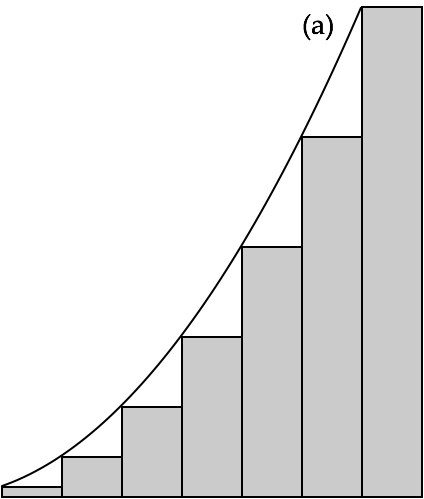
\includegraphics[scale=0.3]{FiguresMaths/SumSquaresContinuous1}
}
\caption{The summation $S_2(n) = \sum_{i=1}^n  i^2$ represented by
  the aggregate area of a sequence of unit-width rectangles, and
  bounded above an below by and ``enveloping'' pair of integrals.  The
  integral that provides the upper bound on the sum yields the area
  under the lefthand continuous curve ($a$), namely, $\int_0^n
  \ (x+1)^2 dx$.  The integral that provides the lower bound yields
  the area under the righthand continuous curve ($b$), namely,
  $\int_1^n \ x^2 dx$.}
\label{fig:riemann-n2}
\end{figure}
$S_2(n) = \sum_{i=1}^n  i^2$ using our strategem.  The rectangles
that represent the respective addends have respective heights heights
$1$, $4$, $9$, $16$, and $25$.  If we were to extend the figure
rightward (to extend the summation and encompass more addends), then
the next rectangle would have height $36$.

\item
In Fig.~\ref{fig:riemann-harmonic1} and~\ref{fig:riemann-harmonic2}, we represent the {\em harmonic} sum
\[ S^{(H)}(n) \ = \ \sum_{i=1}^n \ i^{-1} \ = \ \sum_{i=1}^n \ 1/i.
\]
\begin{figure}[htb]
\centerline{
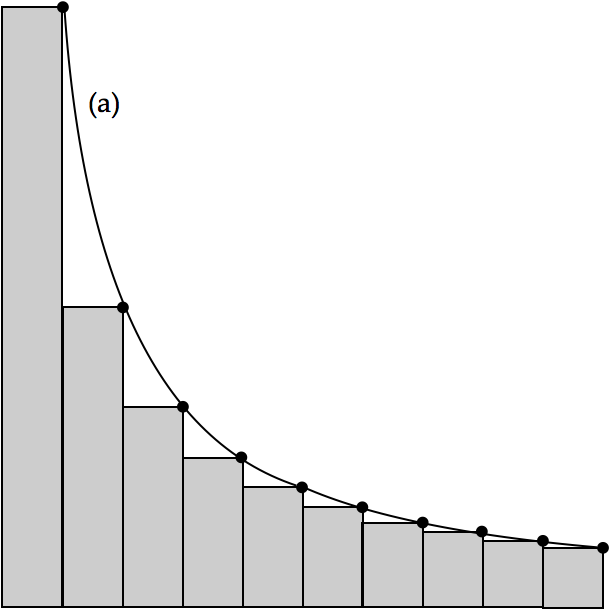
\includegraphics[scale=0.3]{FiguresMaths/RiemannSum1}
}
\caption{The summation $S^{(H)}(n) \ = \ \sum_{i=1}^n \ 1/i$
  represented by the aggregate area of a sequence of unit-width
  rectangles, and bounded above an below by an ``enveloping'' pair of
  integrals.  
  {\Denis the sum is the area of the grey rectangles fo heights 1, 1/2, 1/3, etc.}
  The integral that provides the upper bound on the sum
  yields the area under the righthand continuous curve ($a$), namely,
  $\displaystyle \int_1^n \ \frac{1}{x} dx$. }
%  The integral that
%  provides the lower bound yields the area under the lefthand
%  continuous curve ($b$), namely, $\displaystyle \int_0^{n-1}
%  \ \frac{1}{x+1} dx$.}
\label{fig:riemann-harmonic1}
\end{figure}

\begin{figure}[htb]
\centerline{
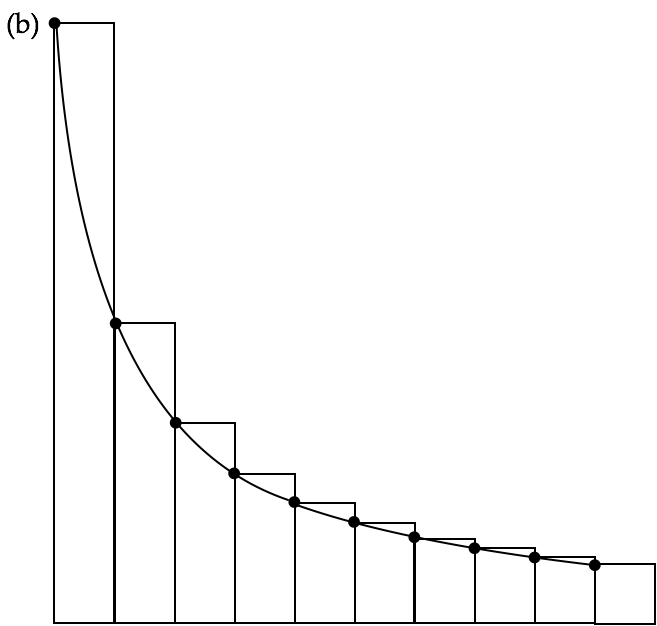
\includegraphics[scale=0.3]{FiguresMaths/RiemannSum2}
}
\caption{ The integral that
  provides the lower bound yields the area under the lefthand
  continuous curve ($b$), namely, $\displaystyle \int_0^{n-1}
  \ \frac{1}{x+1} dx$.}
\label{fig:riemann-harmonic2}
\end{figure}

%
%{\Denis We should add in the caption the explanation of curves (a) and (b)}
%The rectangles that represent the respective addends have respective
%heights $12$, $6$, $4$, $3$, $16/3$, and $2$.  If we were to extend
%the figure rightward (to extend the summation and encompass more
%addends), then the next rectangle would have height $16/7$.
  \end{itemize}

\item
Construct a continuous curve $\overline{C}(x)$ that passes through the
upper {\em lefthand} corners of the unit-width rectangles specified by the
summation.  When constructed appropriately, the area subtended by the
abutting rectangles lies completely under this curve; hence, the area
under the continuous curve---which we obtain by integrating
$\overline{C}$---affords {\em an upper bound} on the summation of interest.

\item
Construct a continuous curve $\underline{C}(x)$ that passes through
the upper {\em righthand} corners of the unit-width rectangles
specified by the summation.  When constructed appropriately, the area
under the curve $\underline{C}(x)$ lies completely within the area
subtended by the abutting rectangles; hence, the area under the
continuous curve---which we obtain by integrating
$\underline{C}$---affords {\em a lower bound} on the summation of
interest.
\end{enumerate}

In the next subsection, we illustrate this strategem using summations
of fixed powers of successive integers---i.e., summations of the form
$\displaystyle S_c(n) \eqdef \sum_{i=1}^n i^c$---for various (classes
of) values of the fixed parameter $c$.


\subsection{Sums of Fixed Powers of Consecutive Integers: $\sum i^c$}
\label{sec:sum-of-i2c}

We obtain bounds on the summations $S_c(n)$ that are rather good for
large values of $n$.  In special cases, our bounds are good, sometimes
even exact, for all values of $n$.

\subsubsection{$S_c(n)$ for general {\em nonnegative} real $c$th powers}
\label{sec:sum-of-i2c>0}

We begin to illustrate the technique of bounding summations via
integrals by focusing on summations of the form
\[ S_c(n) \ \eqdef \ \sum_{i=1}^n \ i^c, \]
for arbitrary positive numbers $c$.  The reader can garner intuition
for the upcoming bounds from the general shape of the rectangles and
continuous curves in Fig.~\ref{fig:riemann-n2}.  We obtain our upper
bound on $S_c(n)$ by evaluating the integral that yields the area
$\overline{C}_c(n)$ under the lefthand continuous curve ($a$) in
Fig.~\ref{fig:riemann-n2}, namely,
\begin{eqnarray}
\label{eq:upper-integral-xc}
\overline{C}_c(n) \ = \
\int_0^n \ (x+1)^c dx & = &
%  \int_0^n \ x^2 dx \ + \ 2 \int_0^n \ x dx \ + \ \int_0^n \ dx \\
% & = & \frac{1}{3} n^3 \ + n^2 \ + \ n \ + \ O(1).
 \frac{1}{c+1} (n+1)^{c+1} \ + \ O(1) \\
\nonumber
 & = & \frac{1}{c+1} n^{c+1} \ + \ O(n^c).
\end{eqnarray}
We obtain our lower bound on $S_c(n)$ by evaluating the integral that
yields the area $\underline{C}_c(n)$ under the righthand continuous
curve ($b$) in the figure, namely,
\begin{equation}
\label{eq:lower-integral-xc}
\underline{C}_c(n) \ = \
\int_1^n \ x^c dx \ = \ \frac{1}{c+1} n^{c+1} \ + \ O(1).
\end{equation}
Combining these bounds, we finally have the following two-sided bound
on $S_c(n)$.
\begin{equation}
\label{eq:bounds-sum-xc}
\frac{1}{c+1} n^{c+1} \ + \ O(1)
  \ \ \leq \ \ S_c(n)
  \ \ \leq \ \ \frac{1}{c+1} n^{c+1} \ + \ O(n^c).
\end{equation}
The main message here is:
\begin{center}
{\em The behavior of $S_c(n)$ is dominated by $\displaystyle
  \frac{1}{c+1} n^{c+1}$ as $n$ grows without bound.  }
\end{center}


\subsubsection{Nonnegative integer $c$th powers}
\label{sec:positive-integer-power}

\paragraph{\small\sf A. A better bound via the Binomial Theorem}

When $c$ is a positive integer, the following special case of Newton's
{\it Binomial Theorem}.\footnote{The general form of the Binomial
  Theorem expands the polynomial $(x+y)^k$ rather than $(x+1)^k$.  See
Section~\ref{sec:Binomial-thm}.}
\index{The Binomial Theorem!restricted form}
affords us a much more detailed version of the upper bound
(\ref{eq:upper-integral-xc})
%(\ref{eq:bounds-sum-xc})
on the sum $S_c(n)$.

\begin{theorem}[The Restricted Binomial Theorem]
\label{thm:restricted-binomial-thm}
For all positive integers $k$,\footnote{See (\ref{eq:binom-coeff}) for
  the definition of, and notation for, the binomial coefficient
  $\displaystyle {k \choose i}$.}
\[ (x+1)^k \ = \
\sum_{i=0}^k \ \ {k \choose i} x^{k-i}.
\]
\end{theorem}

We obtain our improved upper bound on $S_c(n)$ by parallelling the
reasoning that led us to the relation (\ref{eq:upper-integral-xc}).
Our improved upper bound emerges also by evaluating the integral that
yields the area $\overline{C}_c(n)$ under the continuous curve that
passes through the upper lefthand corners of the unit-width rectangles
specified by summation $S_c(n)$.
\begin{eqnarray}
\label{eq:upper-integral-xk}
\overline{C}_c(n) \ = \
\int_0^n \ (x+1)^c dx & = &
\int_0^n \ \left(
\sum_{i=0}^c \ \ {c \choose i} x^{c-i} \right) dx \\
\nonumber
  & = &
\sum_{i=0}^c \ \ \frac{1}{c-i+1} {c \choose i} n^{c-i+1} \ + \ O(1)
\end{eqnarray}
This is a proper upper bound because the region defined by this curve
totally contains the region subtended by the rectangles.

\noindent
Using this strategy, we find that for any positive integer $c$,
summation $S_c(n)$ enjoys the following two-sided bound:
\begin{equation}
\label{eq:bounds-sum-xk}
\frac{1}{c+1} n^{c+1} \ + \ O(1)
  \ \ \leq \ \ \sum_{i=1}^n \ i^c
  \ \ \leq \ \ 
\sum_{i=0}^c \ \ \frac{1}{c-i+1} {c \choose i} n^{c-i+1} \ + \ O(1)
\end{equation}

We have, of course, not changed the dominant behavior of $S_c(n)$ as
$n$ grows without bound, but we have taken a substantial step toward
developing explicit expressions for the summations $S_c(n)$ when $c$
is a positive integer.

\medskip

\paragraph{\small\sf B. Using {\em undetermined coefficients} to
  refine sums}

We now introduce the {\em Method of Undetermined Coefficients}
\index{Method of Undetermined Coefficients}
and illustrate how to use it to derive explicit expressions for the
sums $S_c(n)$ when $c$ is a positive integer.  Our development builds
on the intuition garnered from the bounds (\ref{eq:bounds-sum-xk})
that
\[ S_c(n) \ = \ \frac{1}{c+1} n^{c+1} \ + \ a^{(c)}_c n^c \ + \
a^{(c)}_{c-1} n^{c-1} \ + \ \cdots \ + \ a^{(c)}_2 n^2 \ + \ a^{(c)}_1 n
 + \ a^{(c)}_0
\]
for some nonnegative numbers  $a^{(c)}_{c+1}$, $a^{(c)}_c$, \ldots,
$a^{(c)}_0$.  To begin, we know that $a^{(c)}_0 = 0$, because $S_c(0)
= 0$.
\begin{quote}
{\em Because we are beginning with a conjecture based on intuition, we
  will have to verify the explicit expressions that we derive.  We do
  this after deriving our expressions.}
\end{quote}

Because the Method becomes computationally cumbersome for large values
of $c$, we introduce the reader to it via the first few integer values
of $c$.

{\it The case $c=1$.}
%
We begin with the sum $S_1(n)$, whose value we already know.
Reasoning from the case $c=1$ of (\ref{eq:bounds-sum-xk}), we intuit
that
\[ S_1(n) \ = \ \frac{1}{2} n^2 \ + \ a^{(1)}_1 n \]
for some positive {\it undetermined coefficient} $a^{(1)}_1$.  We can
discover the value of the single unknown, $a^{(1)}_1$ by evaluating
$S_1(n)$ at any single value for the variable $n$.  Any value of $n$
will work; using the {\em smallest} one, $n=1$, simplifies our
calculation.

Because $S_1(1) = 1$, we have
\[ S_1(1) \ = \ 1 \ = \ \frac{1}{2} \ + \ a^{(1)}_1. \]
Therefore, $a^{(1)}_1 = 1/2$, which gives us yet one more derivation
of the value
\[ S_1(n) \ = \ \frac{1}{2} \left( n^2 + n \right) \ = \ 
\frac{n(n+1)}{2}.
\]

\medskip

{\it The case $c=2$.}
%
We derive an explicit expression for $S_2(n) \ \eqdef \  1 + 4 +
\cdots + n^2$.

\begin{prop}
{\em For all} $n \in \N$,
\begin{equation}
\label{eq:sum-1-to-nsq}
S_2(n) \ \eqdef \ \sum_{i=1}^n \ i^2 
 \ = \ \frac{1}{3} n^3 \ + \ \frac{1}{2} n^2 \ + \ \frac{1}{6} n
\end{equation}
\end{prop}

\noindent
$S_2(n)$ is often expressed in a more aesthetic form:
\[ S_2(n) \ = \
\frac{1}{6} n (n+1)(2n+1) \ = \
\frac{2n+1}{3} \cdot {n \choose 2}.
\]

\begin{proof}
Reasoning from the case $c=2$ of (\ref{eq:bounds-sum-xk}), we
propose the conjecture that
\begin{equation}
\label{eq:symbolic-cubic}
S_2(n) \ \ = \ \
\sum_{i=0}^n \ i^2 \ \ = \ \ \frac{1}{3} n^3 + a^{(2)}_2 n^2 + a^{(2)}_1 n.
\end{equation}
for some positive {\it undetermined coefficients} $a^{(2)}_2$ and
$a^{(2)}_1$.  We thereby express $S_2(n)$ as a polynomial in two
unknowns, $a^{(2)}_2$ and $a^{(2)}_1$.  We can determine values for
the unknowns by instantiating the polynomial with (any) two values of
$n$; to simplify calculations, we select the smallest two values of
$n$, namely, $n = 1,2$.  These instantiations of the polynomial leave
us with the following pair of linear equations.
\[
\begin{array}{cccccl}
n=1: & \sum_{i=0}^1 \ i^2
   & = & 1 & = &
1/3 \ + \ a^{(2)}_2 \ + \ a^{(2)}_1 \\
 & & & & & \\
n=2: & \sum_{i=0}^2 \ i^2
   & = & 5 & = &
8/3 \ + \ 4 a^{(2)}_2 \ + \ 2 a^{(2)}_1
\end{array}
\]
By elementary arithmetic, these equations simplify to yield the pair
\[
\begin{array}{ccc}
a^{(2)}_2 \ + \ a^{(2)}_1   & = & 2/3 \\
 & & \\
2 a^{(2)}_2 \ + \ a^{(2)}_1 & = & 7/6
\end{array}
\]
These equations reveal that
\[ 2/3 \ - \ a^{(2)}_2 \ = \ 7/6 \ - \ 2 a^{(2)}_2 \]
so that 
\[ a^{(2)}_2 \ = \ 1/2 \]
which means that
\[ a^{(2)}_1 \ = \ 1/6. \]
We have, thus, derived equation~(\ref{eq:sum-1-to-nsq}).  
\end{proof}

\medskip

We verify our expressions for $S_1(n)$ and $S_2(n)$ by induction in
subsection C.

\medskip

With more (calculational) work, but no new (mathematical) ideas, one
can derive explicit expressions for the sum of the first $n$ $c$th
powers, i.e., the sum $S_c(n)$, for any positive integer $c$.


\medskip

\paragraph{\small\sf C. Validating approximate summations via induction}

We employ the proof technique of (Finite) Induction by proving the
correctness of three summation formulas that have occupied our
attention in this chapter:
\begin{enumerate}
\item
the sum $S_1(n)$ of the first $n$ positive integers; cf., equation
(\ref{eq:sum-1-to-n})

\item
the sum $S_2(n)$ of the squares of the first $n$ positive integers;
cf., equation (\ref{eq:sum-1-to-nsq})

\item
the sum of the first $n$ odd positive integers; cf.,
Proposition~\ref{thm:squares-odd-integers-Gauss}.
\end{enumerate}
We deal with these formulas in turn.

\noindent {\it 1. Verifying equation (\ref{eq:sum-1-to-n}) for $S_1(n)$.}
%
For every positive integer $m$, let {\bf P}$_1(m)$ be the proposition
\[  1 \ + \ 2 \ +  \cdots  + \ m \ = \ {{m+1} \choose 2}. \]
We proceed according to the standard format of an inductive argument.

\begin{description}
\item[{\small\sf The base case P$_1(1)$}.]
%
Because ${\displaystyle {2 \choose 2}} = 1$, proposition {\bf P}$_1(1)$
is true.

\item[{\small\sf The inductive hypothesis}.]
%
Assume, for the sake of induction, that proposition {\bf P}$_1(m)$ is
true for every positive integer $m < n$.  In particular, then,
proposition {\bf P}$_1(n-1)$ is true.

\item[{\small\sf Extending the induction}.]
%
Because proposition {\bf P}$_1(n-1)$ is true, we know that
\[ S_1(n-1) \ = \ 1 + 2 + \cdots + (n-1) \ = \ {n \choose 2}.  \]
By direct calculation, then,
\begin{eqnarray*}
S_1(n) & = & {n \choose 2} + n \\
  & = & \frac{n(n-1)}{2}  \ + \ n \\ 
%  & = & \frac{n^2 - n + 2n}{2} \\
  & = & \frac{n^2 + n}{2} \\
  & = & {{n+1} \choose 2},
\end{eqnarray*}
as was verified in equation (\ref{eq:sum-1-to-n}).
\end{description}
Because $n$ is an arbitrary positive integer, we conclude that
{\bf P}$_1(n)$ is true whenever
\begin{itemize}
\item
{\bf P}$_1(1)$ is true
\item
{\em and}
{\bf P}$_1(m)$ is true for all $m < n$.
\end{itemize}
By the Principle of (Finite) Induction, then, we conclude that
proposition {\bf P}$_1(n)$ is true for all positive integers $n$.
\qed

\bigskip


\noindent {\it 2. Verifying equation (\ref{eq:sum-1-to-nsq}) for $S_2(n)$.}
%
For every positive integer $m$, let {\bf P}$_2(m)$ be the proposition
\[  1 \ + \ 2^2 \ + \ 3^2 \ + \cdots + \ m \ = \ 
\frac{1}{6} m (m+1)(2m+1).
\]
We proceed according to the standard format of an inductive argument.

\begin{description}
\item[{\small\sf The base case P$_2(1)$}.]
%
Because ${\displaystyle \frac{1}{6} (2 \cdot 3)} = 1$, proposition {\bf
    P}$_2(1)$ is true.

\item[{\small\sf The inductive hypothesis}.]
%
Assume, for the sake of induction, that proposition {\bf P}$_2(m)$ is
true for every positive integer $m < n$.  In particular, then,
proposition {\bf P}$_2(n-1)$ is true.

\item[{\small\sf Extending the induction}.]
%
Because proposition {\bf P}$_2(n-1)$ is true, we know that
\[ S_2(n-1) \ = \
\frac{1}{6} (n-1) \cdot n \cdot (2n-1).
\]
By direct calculation, then,
\begin{eqnarray*}
S_2(n) & = &
\frac{1}{6} (n-1) \cdot n \cdot (2n-1) \ + \ n^2 \\
  & = &
\frac{n}{6} \left( (n-1) \cdot (2n-1) + 6n \right) \\
  & = & \frac{n}{6} \left( 2n^2 +3n + 1 \right) \\ 
  & = & \frac{n}{6} (n+1)(2n+1),
\end{eqnarray*}
as was verified in equation (\ref{eq:sum-1-to-nsq}).
\end{description}
Because $n$ is an arbitrary positive integer, we conclude that
{\bf P}$_2(n)$ is true whenever
\begin{itemize}
\item
{\bf P}$_2(1)$ is true
\item
{\em and}
{\bf P}$_2(m)$ is true for all $m < n$.
\end{itemize}
By the Principle of (Finite) Induction, then, we conclude that
proposition {\bf P}$_2(n)$ is true for all positive integers $n$.
\qed


\bigskip

\noindent {\it 3. Verifying that each perfect square $n^2$ is
  the sum of the first $n$ odd integers.}
%
We turn finally to the assertion that, for every positive integer $n$,
\[ n^2 \ = \ 1 \ + \  3 \ + \ 5 \ + \cdots + \ 2n-1. \]
For each positive integer $n$, let {\bf P}$(n)$ denote the proposition
that the preceding equation holds.

The following inductive proof complements the constructive proofs of
the same result in Proposition~\ref{thm:squares-odd-integers-Gauss}.
We proceed according to the standard format of an inductive argument.

\begin{description}
\item[{\small\sf The base case P$(1)$}.]
%
Because $1$ is a perfect square, proposition {\bf P}$(1)$ is true.

\item[{\small\sf The inductive hypothesis}.]
%
Assume, for the sake of induction, that proposition {\bf P}$(m)$ is
true for every positive integer $m < n$.  In particular, then,
proposition {\bf P}$(n-1)$ is true.

\item[{\small\sf Extending the induction}.]
%
Because proposition {\bf P}$(n-1)$ is true, we know that
\[ (n-1)^2 \ = \
 1 + 3 + 5 + \cdots + 2n-3 + 2n-1 \ = \ (n-1)^2 + 2n-1.  \]
By direct calculation, we see that
\[ (n-1)^2 + 2n-1 \ = \ (n^2 -2n +1) + (2n-1) \ = \ n^2. \]
\end{description}
Because $n$ is an arbitrary positive integer, we conclude that
{\bf P}$(n)$ is true whenever
\begin{itemize}
\item
{\bf P}$(1)$ is true
\item
{\em and}
{\bf P}$(m)$ is true for all $m < n$.
\end{itemize}
By the Principle of (Finite) Induction, then, we conclude that {\bf
  P}$(n)$ is true for all $n \in \N^+$.
\qed


\subsubsection{$S_c(n)$ for general {\em negative} $c$th powers}
\label{sec:sum-of-i2c<0}

We focus finally on summations of the form
\[ S_c(n) \ \eqdef \ \sum_{i=1}^n \ i^c, \]
for arbitrary {\em negative} numbers $c$.  The reader can garner
intuition for the upcoming bounds from the general shape of the
rectangles and continuous curves in Fig.~\ref{fig:riemann-harmonic}.
We obtain our upper bound on $S_c(n)$ by evaluating the integral that
yields the area $\overline{C}_c(n)$ under the righthand continuous
curve ($a$) in that figure, and We obtain our lower bound on $S_c(n)$
by evaluating the integral that yields the area $\underline{C}_c(n)$
under the lefthand continuous curve ($b$) in that figure.  We thereby
find that
\begin{equation} 
\label{eq:general-bounds-negative-xc}
\left[
\underline{C}_c(n) \ = \
\int_0^{n-1} \ (x+1)^c dx
\right]
\ \leq \ S_c(n) \ \leq \
\left[
\overline{C}_c(n) \ = \
\int_1^n \ x^c dx
\right].
\end{equation}

When $c \neq -1$,\footnote{We need to avoid the case $c = -1$ so that
  we do not attempt to divide by $0$.}~we can provide more detail,
using reasoning similar to that underlying the bounds
(\ref{eq:bounds-sum-xc}) that hold for positive values of $c$.

\paragraph{\small\sf A. Negative powers $c$ with $-1 < c < 0$}

In this case, we obtain essentially the same bounds as in the case of
nonnegative $c$.  To wit,
\begin{equation}
\label{eq:bounds-(-1)<c<0}
\begin{array}{l}
\mbox{For $-1 < c< 0$:} \\
 \\
\hspace*{.35in}
{\displaystyle \frac{1}{c+1} n^{c+1} \ - \ O(n^c)}
  \ \ \leq \ \ S_c(n)
  \ \ \leq \ \
{\displaystyle \frac{1}{c+1} n^{c+1} \ + \ O(1)}.
\end{array}
\end{equation}
We thus observe that $S_c(n)$ has the same growth {\em pattern} as $n$
grows as it does when $c$ is positive, but that $S_c(n)$'s growth {\em
  rate} is slower because of the damping effect the negative $c$ in
the exponent.

\paragraph{\small\sf B. Negative powers $c$ with $c < -1$}

When $c$ is ``very negative''---specifically, when $c < -1$---then we
encounter {\em convergent infinite series}.  Because $n^c$ {\em
  shrinks} in this case as $n$ grows, an analysis mirroring the one
that leads to (\ref{eq:bounds-(-1)<c<0}) provides the following sum
for the infinite version of $S_c(n)$, call it $S_c^{(\infty)}$.

\begin{equation}
\label{eq:bounds-negative-(not-1)-sum-xc}
\begin{array}{l}
\mbox{For $c<-1$, as $n$ grows without bound:} \\
 \\
\hspace*{.35in}
S_c^{(\infty)} \ \ \mbox{ tends to the value } \ \
{\displaystyle \frac{1}{c+1}}
\end{array}
\end{equation}

\paragraph{\small\sf C. Negative powers $c$ with $c = -1$: the {\em harmonic} sum}

The singular case defined by the value $c = -1$ defines the important
{\it harmonic series} and its finite prefixes, the {\it harmonic sums}.
\begin{equation}
\label{eq:harmonic}
\begin{array}{lcll}
S^{(H)} & = & {\displaystyle \sum_{i=1}^\infty \ \frac{1}{i}} & \hspace*{.25in}
  \mbox{the full harmonic series} \\
S^{(H)}(n) & = & {\displaystyle \sum_{i=1}^n \ \frac{1}{i} } & \hspace*{.25in}
  \mbox{the $n$-term harmonic sum} \\
\end{array}
\end{equation}

It has been known since the time of the well-traveled Swiss
mathematician Leonhard Euler
\index{Euler, Leonhard}
that $S^{(H)}(n) \ \approx \ \ln n$, where $\ln n$ is the logarithm
whose base is Euler's constant
\index{Euler's constant}
$e = 2.718281828 \ldots$

\begin{quote}
{\em The adjective ``harmonic'' calls to mind a number of cancepts
  associated with {\em music}, such as ``harmonics'' and ``harmony''.
  The association between our series and these musical concepts is not
  a coincidence.  The name of the harmonic series derives from the
  concept of {\em overtones}, or {\em harmonics}, in music.  When one
  observes a vibrating string, one finds that the wavelengths of its
  overtones, as fractions of the string's fundamental wavelength, are
  the terms of the {\em harmonic sequence}, namely, $\frac{1}{2}$,
  $\frac{1}{3}$, $\frac{1}{4}$, \ldots.  }
\end{quote}








\ignore{********************
\subsection{Deriving and Solving Linear Recurrences}
\label{sec:linear-recurrences-2}

We have discussed already discussed the use of linear recurrences in
Section~%PLACE REFERENCE TO \ref{sec:linear-recurrences-1}.
 We now derive the mathematics
underlying this important topic.

By the time the reader has reached this paragraph, she has the
mathematical tools necessary to prove and apply what is called {\it
  The Master Theorem for Linear Recurrences} \cite{CLRS}.  This level
of mathematical preparation should be adequate for most
early-undergrad courses on data structures and algorithms, as well for
for analyzing a large fraction of the algorithms that she is likely to
encounter in daily activities.

\noindent {\bf Theorem}[The Master Theorem for Linear Recurrences]
\label{thm:master-thm}
%\index{The Master Theorem for Linear Recurrences}
{\it 
Let the function $F$ be specified by the following linear recurrence.}
\begin{equation}
\label{eq:Lin-Recur:start}
F(n) \ = \ \left\{
\begin{array}{cl}
a F(n/b) + c & \mbox{for } n \geq b \\
c & \mbox{for } n < b
\end{array}
\right.
\end{equation}
{\it
Then the value of $F$ on any argument $n$ is given by}
\begin{equation}
\label{eq:Lin-Recur:solve}
\begin{array}{lclll}
F(n) & = & (1 + \log_b n)c &  & \mbox{if } a=1 \\
     &   &                 &  & \\
     & = &
  {\displaystyle
  \frac{1-a^{\log_b n}}{1-a} \ \approx \ \frac{1}{1-a}
  }
 &  & \mbox{if } a<1 \\
    &   &                  & & \\
    & = &
  {\displaystyle
\frac{a^{\log_b n} -1}{a-1}
  }
 & & \mbox{if } a>1
\end{array}
\end{equation}


\begin{proof}
In order to discern the recurring pattern in
(\ref{eq:Lin-Recur:start}), let us begin to ``expand'' the specified
computation by replacing occurrences of $F(\bullet)$ as mandated in
(\ref{eq:Lin-Recur:start}).
\begin{equation}
\label{eq:Lin-Recur:expand}
\begin{array}{lcccc}
F(n) & = & a F(n/b) + c & & \\
     & = & a \left( a F(n/b^2) + c \right) + c
             & = & a^2 F(n/b^2) + (1 + a)c \\
     & = & a^2 \left( a F(n/b^3) + c \right) + (1+a)c
             & = & a^3 F(n/b^3) + (1 + a + a^2)c \\
     &   & \vdots & & \vdots \\
     & = & 
{\displaystyle
\left( 1 + a + a^2 + \cdots + a^{\log_b n} \right) c
} & &
\end{array}
\end{equation}
The segment of (\ref{eq:Lin-Recur:expand}) ``hidden'' by the vertical
dots betokens an induction that is left to the reader.  Equations
(\ref{eq:geom-sum:b>1}) and (\ref{eq:geom-sum:b<1}) now enable us to
demonstrate that (\ref{eq:Lin-Recur:solve}) is the case-structured
solution to (\ref{eq:Lin-Recur:start}).
\end{proof}
********************}

